Atualmente, a tecnologia é um fator chave quando se trata do processo criativo do design gráfico. A variedade de ferramentas a disposição do designer e sua eficiência são necessárias para atender de forma ideal as demandas do mercado. Nesta seção, como o software uEye se destaca no mercado de ferramentas e como ele se compara com outras tecnologias.


O primeiro estudo, conduzido por \textcite{GEORGES2016}, busca desenvolver uma ferramenta de avaliação para UX que utiliza rastreamento ocular e sinais psicológicos e comportamentais para criar heatmaps das interações do usuário com um sistema. Esses heatmaps não apenas mostram onde o usuário fixa o olhar durante a interação, mas também associam essas áreas aos estados emocionais do usuário.

Para a criação dos mapas de calor, foram empregados diversos processos, por exemplo, a triangulação de dados, que por sua vez foi realizada sincronizando as informações de rastreamento ocular com sinais fisiológicos, como frequência cardíaca e atividade elétrica da pele, o que possibilitou a obtenção de dados sobre o estado emocional do usuário. Além disso, um modelo de aprendizado de máquina foi utilizado para estimar a atividade cognitiva com base nos sinais fisiológicos, permitindo que os heatmaps não só identifiquem as áreas mais visualizadas, mas também indiquem aquelas que geram maior sobrecarga mental. 

Todos os dados gerados por esse processo passaram por uma etapa de normalização e colorização, na qual as áreas de interesse foram destacadas com cores proporcionais à intensidade dos estados psicológicos associados.

O experimento descrito no artigo envolveu 26 participantes, com a meta de analisar a carga cognitiva em relação à complexidade visual de interfaces de sites. Para o estudo, os pesquisadores selecionaram nove páginas iniciais de websites, distribuídas em três níveis de complexidade visual: baixo, médio e alto. Essas interfaces foram projetadas para induzir diferentes níveis de carga cognitiva nos usuários. As interfaces com maior complexidade visual exigiram mais recursos cognitivos, confirmando uma correlação direta entre a complexidade percebida e a carga cognitiva experimentada.

\begin{photograph}[H]
    \centering
    \SetCaptionWidth{\ifbool{@LayoutA}{0.7}{0.72}\linewidth}
    \caption{Heatmap do uso cognitivo de três complexidades de telas}%
    \label{phot:}
    \savebox0{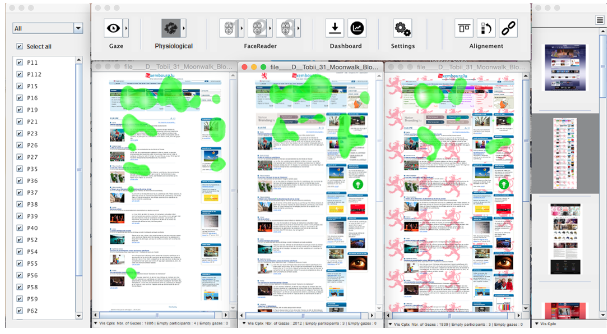
\includegraphics[width = \CaptionWidth]{Illustrations/georges.png}}
    \usebox0%
    \SourceOrNote{GEORGES2016}
    \end{photograph}


Os resultados mostraram que os heatmaps fisiológicos, correlacionaram-se significativamente com as avaliações subjetivas dos usuários em relação à complexidade visual das interfaces. Esses heatmaps se destacaram ao capturar com precisão as áreas com maior demanda cognitiva nas interfaces, superando as formas tradicionais de mapear o rastreamento ocular em termos de precisão na predição da carga cognitiva.

O estudo conduzido por \textcite{SOUZA2021} propõe um framework de avaliação de UX que combina rastreamento ocular, monitoramento de movimentos do mouse e entradas do teclado, além de inteligência artificial, para categorizar o desempenho de usuários em sistemas de informação. Esse framework, chamado AIT2-UX, analisa a experiência do usuário com base em diferentes fontes de dados, fornecendo sobre a usabilidade e interação dos usuários com interfaces digitais.

Para implementar o AIT2-UX, a coleta de dados foi realizada em um processo que incluiu variáveis de rastreamento ocular, de movimento do mouse e de uso do teclado. Essas variáveis foram armazenadas na forma de mapas de calor e gráficos de interação, permitindo identificar áreas específicas onde os usuários enfrentaram dificuldades. Além disso, modelos de aprendizado de máquina foram utilizados para classificar os usuários como “experientes” ou “não-experientes”, com base em padrões extraídos das variáveis de interação e dos questionários de usabilidade realizados. A árvore de decisão foi o modelo que apresentou o melhor desempenho, com uma acurácia de 94\% ao capturar as características de interação do usuário, indicando seus diferentes níveis de experiência.

Para a geração dos mapas de calor, foi utilizada a ferramenta T2-UXT, que registrou as interações dos usuários com o site da Receita Federal do Brasil (RFB) ao realizarem tarefas como acesso a serviços do CPF e localização de páginas específicas. Esses mapas de calor revelaram áreas onde os usuários com diferentes níveis de experiência focavam a atenção, mostrando que os usuários menos experientes gastam mais tempo e realizam mais movimentos de busca na interface, sinalizando que o layout do site apresenta dificuldades ao usuário para completar tarefas de forma eficiente.

Os resultados sugerem que o framework AIT2-UX e a ferramenta T2-UXT podem fornecer informações detalhadas para aprimorar o design de interfaces com base no comportamento do usuário. Além disso, o estudo propôs customizações para o site da RFB que poderiam facilitar a navegação, como destacar automaticamente áreas de interesse com base no perfil do usuário. Esses insights demonstram o potencial do framework para melhorar a experiência do usuário em ambientes digitais, oferecendo uma solução que pode ser aplicada para a melhora da experiência de usuários em diferentes sistemas.

\begin{photograph}[H]
    \centering
    \SetCaptionWidth{\ifbool{@LayoutA}{0.7}{0.72}\linewidth}
    \caption{Heatmap do mouse tracking aplicado ao site da RFB}%
    \label{phot:}
    \savebox0{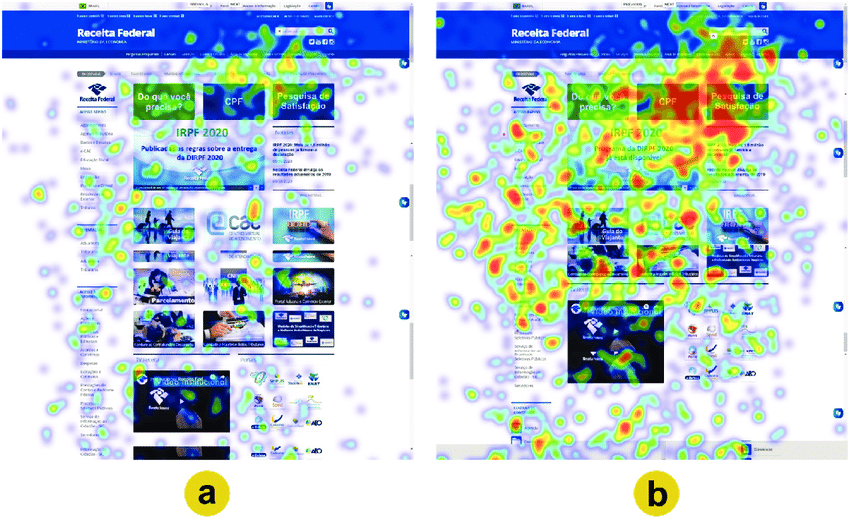
\includegraphics[width = \CaptionWidth]{Illustrations/Heat-map-mouse-tracking-a-profile-1-b-profile-2.png}}
    \usebox0%
    \SourceOrNote{SOUZA2021}
    \end{photograph}
